\documentclass[11pt,english,openright]{book}
\usepackage[a4paper]{geometry}
\usepackage[english]{babel}
\usepackage{fancyhdr}
\usepackage{float}
\usepackage{setspace}
\usepackage{epsfig}
\usepackage{indentfirst}
\usepackage[normalem]{ulem}
\usepackage[table]{xcolor}
\usepackage{algpseudocode}
\usepackage{smartdiagram}
\usepackage{listings}
\usepackage{changepage}   % for the adjustwidth environment
\usepackage{tipa}
\usepackage{coloremoji}
\usepackage{tikz}
\usepackage{tabularx}

% DELETE ME BELOW
\usepackage{blindtext}
% DELETE ME ABOVE


\usepackage[unicode=true,pdfusetitle,
 bookmarks=true,bookmarksnumbered=false,bookmarksopen=false,
 breaklinks=false,pdfborder={0 0 0},backref=false,colorlinks=false]
 {hyperref}

\makeatletter
% spacing
\onehalfspacing

% geometry
\geometry{verbose,tmargin=3cm,bmargin=3.5cm,lmargin=4cm,rmargin=3cm, nomarginpar}
\setcounter{secnumdepth}{3}
\setcounter{tocdepth}{3}

% pdf properties
\hypersetup{pdftitle={Working title}, pdfauthor={Milica Jovanović, Mirjam Škarica}}

% set page page count from the first chaprer's page
\fancypagestyle{plain}{
\fancyhead{}
\renewcommand{\headrulewidth}{0pt}
\renewcommand{\footrulewidth}{0pt}
\fancyfoot{\begin{flushright}\thepage\end{flushright}}
}

% prettify headers for the thesis
\fancyhead{}
\fancyhead[LE]{\slshape \nouppercase \leftmark}
\fancyhead[RO]{\slshape \nouppercase \rightmark}
\fancyfoot{\begin{flushright}\thepage\end{flushright}}
\renewcommand{\headrulewidth}{0.4pt}
\setlength{\headheight}{14pt}

\@ifundefined{showcaptionsetup}{}{
\PassOptionsToPackage{caption=false}{subfig}}



\definecolor{darkgray}{gray}{0.2}
\definecolor{lightgray}{gray}{0.8}
\definecolor{bblue}{HTML}{5C9BD1}
\definecolor{rred}{HTML}{F6A561}
\definecolor{ggreen}{HTML}{78B7B2}
\definecolor{ppurple}{HTML}{9D68A9}
\pgfplotsset{compat=1.12} 
\usetikzlibrary{pgfplots.groupplots}

\newcommand{\lcb}{{\tt {\char '173}}}
\newcommand{\rcb}{{\tt {\char '175}}}

% centered column for tabularx
\newcolumntype{C}{>{\centering\arraybackslash}X}

% header for tabularx
\newcommand*{\thead}[1]{\multicolumn{1}{c}{\bfseries #1}}

% inline code 
\newcommand{\inlinecode}{\texttt}

\let\underscore\_
\newcommand{\wrapunderscore}{\renewcommand{\_}{\underscore\hspace{0pt}}}
\wrapunderscore

% personalized commands
\newcommand{\quoted}[1]{``#1''}
\newcommand{\Csh}{C\includegraphics{hash-symbol}}
\makeatother


% --- JSON DEFINITION ---
\newcommand\JSONnumbervaluestyle{\color{blue}}
\newcommand\JSONstringvaluestyle{\color{gray}}

% switch used as state variable
\newif\ifcolonfoundonthisline

\makeatletter

\lstdefinestyle{json}
{
  showstringspaces    = false,
  keywords            = {false,true},
  alsoletter          = 0123456789.,
  morestring          = [s]{"}{"},
  stringstyle         = \ifcolonfoundonthisline\JSONstringvaluestyle\fi,
  MoreSelectCharTable =%
    \lst@DefSaveDef{`:}\colon@json{\processColon@json},
  basicstyle          = \ttfamily,
  keywordstyle        = \ttfamily\bfseries,
}

% flip the switch if a colon is found in Pmode
\newcommand\processColon@json{%
  \colon@json%
  \ifnum\lst@mode=\lst@Pmode%
    \global\colonfoundonthislinetrue%
  \fi
}

\lst@AddToHook{Output}{%
  \ifcolonfoundonthisline%
    \ifnum\lst@mode=\lst@Pmode%
      \def\lst@thestyle{\JSONnumbervaluestyle}%
    \fi
  \fi
  %override by keyword style if a keyword is detected!
  \lsthk@DetectKeywords% 
}

% reset the switch at the end of line
\lst@AddToHook{EOL}%
  {\global\colonfoundonthislinefalse}

\makeatother


\begin{document}
% --- FRONTPAGE ---
\frontmatter
\pagestyle{empty}\pagenumbering{alph}
\newgeometry{margin=3cm}
\pdfbookmark{Front Page}{front-page}
\begin{titlepage}

\begin{center}
\Large{\textsc{Politecnico di Milano}}\\
\Large{Scuola di Ingegneria Industriale e dell'Informazione}\\
\large{Corso di Laurea Magistrale in Ingegneria Informatica}\\
\large{Dipartimento di Elettronica, Informazione e Bioingegneria}
\par\end{center}

\vspace{0.5cm}


\begin{center}
\begin{figure}[h]
\centering{}
\includegraphics[width=0.5\textwidth]{00-frontpage/logo-polimi.png}
\end{figure}
\vspace{1cm}

\par\end{center}

\begin{center}
\LARGE{A framework for comparing open source\\ sentiment analysis APIs}\vspace{2cm}

\par\end{center}

\begin{flushleft}
\begin{tabular}{ll}
Relatore:  & Prof.ssa Letizia TANCA\tabularnewline
Correlatori:
	& Prof.ssa Maristella MATERA\tabularnewline
	& Ing. Riccardo MEDANA
\end{tabular}\vspace{1cm}

\par\end{flushleft}

\begin{flushright}
\begin{tabular}{ll}
Tesi di laurea di: & \tabularnewline
Milica JOVANOVI\'{C} & Matr. 835953\tabularnewline
Mirjam \v{S}KARICA & Matr. 836505\tabularnewline
\end{tabular}\vspace{2.2cm}

\par\end{flushright}

\begin{center}
{\large{}Academic Year 2016\textendash 2017}
\par\end{center}{\large \par}

\end{titlepage}
\restoregeometry

\cleardoublepage{}

%\begin{flushright}
%\emph{
Some nice inspirational and aspirational quote. 
Some nice inspirational and aspirational quote. 
\bigskip

Someone

}\cleardoublepage{}
%par\end{flushright}

% --- CHAPTER SUMMARY ---
\chapter*{Summary}
\thispagestyle{empty}\input{Summary.tex}\cleardoublepage{}

% --- CHAPTER ABSTRACT ---
\chapter*{Abstract}
\thispagestyle{empty}With the rise of social media the way business and customers interact has drastically changed. 
Business are expected to have a web presence and to produce content in order to engage with their user base on a daily base. 
In return, the users don't shy away from leaving feedback, and they leave a lot of it. 

Having that in mind, it is easy to see how having an automated way to tell if the user-generated content was negative or positive would provide a lot of value for a businesses. 
Coincidentally, in recent years a lot of research and advances have been made in the field of sentiment analysis and the efforts yielded a number of tools for predicting sentiment of textual content.
This is why we were interested in examining the landscape of open source APIs that provide that functionality.

In this thesis we have built a framework for assessing the performance of some  open source  APIs for sentiment analysis. 
The APIs were tested against a dataset of social media content generated by real fashion brands and their user base. 
Because of the global nature of the fashion industry the APIs were appraised on how well they perform in predicting  sentiment of data in original language as well as their English translations. 
Finally, the framework improved  the accuracy of procured sentiment predictions by taking into account the sentimental value of emojis and emoticons found in the data.
\cleardoublepage{}

\setcounter{page}{1}\pagenumbering{roman}

\pagestyle{fancy}

% --- CHAPTER TABLE OF CONTENTS ---
\pdfbookmark{Table of contents}{toc}
\tableofcontents{}

% --- CHAPTERS LIST OF FIGURES ---
\listoffigures
% --- CHAPTERS LIST OF TABLES  --- 
\listoftables
% LIST OF ALGIRITHMS ----
%\listof{algorithm}{List of algorithms}

% reset page count & number style
\cleardoublepage{}\mainmatter
\renewcommand{\sectionmark}[1]{\markright{\thesection.\ #1}}
\renewcommand{\chaptermark}[1]{\markboth{\thechapter.\ #1}{}}


% --- CHAPTER INTRODUCTION ---
\chapter{Introduction\label{ch:introduction}}
Some text \cite{masse2011rest} \Blindtext \cite{rizzo2015progettazione}
\Blindtext

\clearpage

\section{Structure}
\blindtext

\begin{itemize}
	\item 
	In the chapter \ref{ch:state-of-the-art} blahblah
	\item 
	In the chapter \ref{ch:sentiment-analysis-workflow} \blindtext

\end{itemize}

% --- CHAPTER STATE OF THE ART ---
\chapter{State of the art\label{ch:state-of-the-art}}
This chapter describes state of the art of sentiment analysis in social media.
Chapter consists of three sections, each of them trying to bring closer the need for sentiment analysis in current market:

\begin{enumerate}
	\item Need for sentiment analysis
	\item Application of sentiment analysis in various companies and non-profit organizations
	\item Some tools for sentiment analysis
\end{enumerate}

\section{Need for sentiment analysis}
With growth of people's interaction and company's advertisements through social media, we have come to the point of realizing that people sharing opinions could help us "predict" stock market and as well follow current trends by guiding the market according to the customers input.
Customers nowadays have endless ways to interact with brands which could help increasing brand's awareness, but if not properly analyzed could also lead to obtaining not quite accurate view of customer's satisfaction.
The idea of analyzing customer opinion has driven companies to search for an automated way of understanding content that are customers sharing online. The main network for spreading opinions is social media. Almost every tweet, comment, re-share or  review gives an information that could guide a company towards better planning, optimizing production and better stock managing.
Reason for finding an automated way of analyzing customer's opinion comes from a problem of big data being generated each day which makes impractical to do manually analysis of each user input. Leaving the big data problem aside, brings us to another issue; being able to beat natural language processing challenge. Reason for making the task harder is that user input might be informal, "slang like" content with emojis , hashtags, full with sarcastic sentences which would lead to unreliable results of analysis.

\section{Application of sentiment analysis in various companies and non-profit organizations}
Customers engagement through social media can be a valuable asset for companies to understand level of acceptability of their products. By finding a way to analyze raw text data and catch the key context from it could potentially result in decrease of stock planning cost and in increase of profit.
Over the years many companies and nonprofit organizations have started applying some kind of data analysis for this purpose. One of current expanding areas of data analysis is the sentiment analysis, this emerging technique has been applied in various spheres. We will give an insight to few representive examples of successful solutions and their consequences.
Cathay Pacific as one of leading airline companies started using one of the commercial solutions for sentiment analysis. They have used Brandwatch platform in order to monitor how their campaign hashtag has been mentioned across social media. Specifically, in which connotation the hashtag has been used, what people talk about when putting it in their posts, which has been show in Cathay Pacific Case Study: Using Social Data to Inform a Global Business \cite{CathayPacific} Aside the sentiment sensing, they are using the platform to identify trends, such as what are people talking about when traveling and where are they traveling to. This kind of data can help them create new ideas for future developments.
Nonprofit organizations like American Cancer Society are using sentiment analysis in order to obtain feedback on organized fund raising event. The difference between this kind of sentiment analysis and the one used by Cathay Pacific is that for ACS a model needs to be trained because words used have another connotation for them. For example, words such as “kill” and “cancer” in case of ACM should have positive sentiment. Sensing on social media has shown that ACM had spikes in user engagement every time there was a big fund-raising event. In order to raise more funds, by data analysis they have realized that doing more announcements before, during and after the event could help them to raise people’s awareness about the problem they are fighting against. The ACS also used sentiment analysis to find out what it should be tweeting and posting. For instance, October is Breast Cancer Awareness month and pink ribbons are everywhere. Some NFL teams even wore pink shoes and gloves to raise awareness cited in How Starbucks And Other Companies Use Complex Math Algorithms To Read Your Feelings Online\cite{Starbucks}.\\

\section{Some tools for sentiment analysis}

\subsection*{Commercial solutions}
As every commercial product, basic goal is user satisfaction. Commercial solutions provide user with rich customizable, easy to use interfaces for a not so fair price. By paying for the service users, usually medium to large scale companies, receive a platform which contains algorithms for data analysis used as a black box and detailed colorful visualization tools for representing results of the analysis. One of important issues that users wouldn’t deal with, as they would if building their own solutions, is that such platforms usually come with needed infrastructure to support such data intense analysis. Here we will mention few most widely used commercial tools.\\
\textit{Google Analytics\\}
Google Analytics helps you know your audience, find your best content, and optimize ad inventory. Providing you with real-time reports of what is happening on your site right now so you can make adjustments fast. Engagement metrics help you see what is working, while integrations with Google and publisher tools like AdSense, DoubleClick AdExchange, and DoubleClick for Publishers (Analytics 360 only) make it easy to package and sell your ad inventory.  Google has developed a solution which enables the user to gather data, preprocess it, and train a model using Google Prediction API like a black box.\\
\textit{Sales Force Marketing Cloud solution - Radian6\\}
Most certainly that human sentiment analysis is the most accurate method even if you think how much human differ in their interpretation. Radian6 has introduced an automated sentiment analysis tool which has flexibility to allow users to change the perspective of analysis. If you do real sentiment evaluation manually, you will obtain more accurate results than any other automated tool could give you. Given a simple example, if a user compares different beverage brands, most likely he would rate better the beverage he prefers based on the prevailing taste of it. Radian6 solution will enable the user to do deeper analysis into specific topics via different types of ad hoc analysis
Radian6 has given various solutions to fill the gap between marketing and customer satisfaction by using social insights to drive marketing campaigns. By listening, engaging and analyzing data on social media, users are able to create sales plans which could lead to better stock planning.\\
\textit{Brandwatch\\}
Brandwatch Analytics is a web-based platform with monthly subscription basis with different range of packages meeting needs of various company sizes. They search and store date based on users queries on the market. Quite accurately guarantees spam free and duplicate free data. With the gathered data they assure you of optimizing marketing in social media. The platform offers various customizations that could accommodate to the needs of the user. By acquiring data every day and providing users with tools to analyze and visualize them, they have convinced a lot of famous brands that Brandwatch is a good tool to help them make data-driven market decisions such as Cisco, British Airways and Dell. 
Good thing about Brandwatch as a commercial solution is that it provides coverage of various data sources, independent of language barrier or data quality. Besides of the coverage advantage, it provides stable analytic tools, as well as visualization tools.  It is mostly used by large companies that could afford the platform.\\
\subsection*{Open source solutions}
Main benefits of adopting an open source solution are lower costs, in this case using an open source library is free, as well as trend of keeping an open source solution always available because it is usually maintained by a community. For a commercial solution, it could happen that a vendor shuts down his business and with it taking its software out of market. Another major advantages of using an open source solution is that often there is a collaboration between libraries and as well as variety of available solutions. Open source solutions are not bind to changes and updates to releases; instead they can be developed collaboratively when functionality is needed. Of course using an open source library can have its down sides, a library or an API call can be limited by number of usages by day or by accepted amount of data it can receive. Thus implicates that these kind of solutions are not setting up an infrastructure that could handle data-intensive analysis and are usually used for educational purposes.\\
\textit{Natural Language Toolkit\\}
Natural Language Toolkit is an open source platform for building programs which work with textual data. It is equipped with various libraries for text processing which provide tokenization, tagging, stemming and handy wrappers around NLP libraries. NLTK has a very detailed documentation which can guide a developer in building an application that suits his needs. Highly recommended for people that feel free working in Python.\\
\textit{Stanford’s CoreNLP\\}
Provide set of tools written in Java for purpose of natural language processing. Initially was built to work only with English language, but latest releases support languages such as Arabic, Chinese, French, German and Spanish. It is an integrated framework easy to use for language manipulation on raw inputted text. The result it gives after initial analysis is a good starting point for building application with domain-specific problems. Besides low level natural language processing, it contains as well some traces of deep learning algorithms.\\
\textit{Text-Processing\\}
The text-processing is an open source API which returns simple JSON over HTTP web service for text mining and natural language processing. It is an API which supports speech tagging, chunking, sentiment analysis, phrase extraction and named entity recognition. As an open source solution it has its limitations, such as 1000 calls per day per IP. 
To get the sentiment of a text, users should do an HTTP request with form encoded data containing text to analyze. As a response, users will receive a JSON object with a label marking the sentiment (can be pos as positive, neg as negative or neutral) and a probability for each label.\\

Searching around Internet about sentiment analysis has shown us that each of the available solutions has it’s strengths and weaknesses. Seeing that APIs behave differently depending on the data or domain applied on, we came to an idea to build a framework that gives an overview of the open source APIs, concluding their advantages and disadvantages, as well as representing comparison between them. Building a framework that is able to invoke different APIs and show sentiment results with statistical representation of accuracy has been a good indicator of choosing an appropriate solution for a specific problem domain.  




% --- CHAPTER SENTIMENT ANALYSIS WORKFLOW ---
\chapter{Sentiment analysis workflow\label{ch:sentiment-analysis-workflow}}
This chapter describes the workflow used to analyze the sentiment of social media comments and their corresponding posts.
In order to outline the workflow, a top down approach was taken where each subsequent section provides an ever more detailed insight into a particular step of the workflow.
The big picture is shown in Figure \ref{fig:analysis-workflow} and consists of four parts:
\begin{enumerate}
  \item Obtaining data
  \item Sentiment prediction using an API
  \item Determining real sentiment of data
  \item Evaluation of that API's performance
\end{enumerate}

The first part is the simplest one and as such doesn't merit a more detailed recounting other than mentioning that we were provided with a small sample dataset which, most relevantly, contained about 6000 comments.

In the sections that follow, each of the three remaining parts are broken down into conceptual steps describing the methodology used whilst not cluttering it with too many implementation details.
Additionally, it is interesting to note that the first and third steps are performed only once.
This means that, for each new API we want to use, the workflow for sentiment analysis effectively consists of only steps 2 and 4, namely sentiment prediction and performance evaluation.


This chapter describes the workflow used to analyze the sentiment of social media comments and their corresponding posts.
In order to outline the workflow, a top down approach was taken where each subsequent section provides an ever more detailed insight into a particular step of the workflow.
The big picture is shown in Figure \ref{fig:analysis-workflow} and consists of four parts:
\begin{enumerate}
  \item Obtaining data
  \item Sentiment prediction using an API
  \item Determining real sentiment of data
  \item Evaluation of that API's performance
\end{enumerate}

The first part is the simplest one and as such doesn't merit a more detailed recounting other than mentioning that we were provided with a small sample dataset which, most relevantly, contained about 6000 comments.

In the sections that follow, each of the three remaining parts are broken down into conceptual steps describing the methodology used whilst not cluttering it with too many implementation details.
Additionally, it is interesting to note that the first and third steps are performed only once.
This means that, for each new API we want to use, the workflow for sentiment analysis effectively consists of only steps 2 and 4, namely sentiment prediction and performance evaluation.


This chapter describes the workflow used to analyze the sentiment of social media comments and their corresponding posts.
In order to outline the workflow, a top down approach was taken where each subsequent section provides an ever more detailed insight into a particular step of the workflow.
The big picture is shown in Figure \ref{fig:analysis-workflow} and consists of four parts:
\begin{enumerate}
  \item Obtaining data
  \item Sentiment prediction using an API
  \item Determining real sentiment of data
  \item Evaluation of that API's performance
\end{enumerate}

The first part is the simplest one and as such doesn't merit a more detailed recounting other than mentioning that we were provided with a small sample dataset which, most relevantly, contained about 6000 comments.

In the sections that follow, each of the three remaining parts are broken down into conceptual steps describing the methodology used whilst not cluttering it with too many implementation details.
Additionally, it is interesting to note that the first and third steps are performed only once.
This means that, for each new API we want to use, the workflow for sentiment analysis effectively consists of only steps 2 and 4, namely sentiment prediction and performance evaluation.


\input{03-sentiment-analysis-workflow/diagrams/sentiment-analysis-workflow.tex}


% --- SECTION PREDICTON WORKFLOW ---
\section{Sentiment prediction workflow\label{sec:sentiment-prediction-workflow}}
Let's assume we have access to an API for sentiment prediction. By having access we mean being able to programmatically call the API with a text payload and have it return a prediction in some data format. The end goal is to analyze sentiment of all the comments in our sample dataset and aggregate the obtained data on a per-post basis in order to infer whether it was positively or negatively received, or even if it had no emotional impact whatsoever. And we want this to be done automatically, practically with a push of a proverbial button. By automatizing the process, it is easy to see how it can derive value for possible future ventures that extend far beyond our modest 6000 comment database.

\input{03-sentiment-analysis-workflow/diagrams/sentiment-prediction-workflow.tex}

Figure \ref{fig:prediction-workflow} shows the main concepts that build up the workflow of our sentiment analysis. 
Since the term \textit{workflow} can be a bit ambiguous, let us clarify exactly what we mean by it. In our case it is simply a python script named \textit{automated\_sentiment\_analysis.py} that can be run manually, or scheduled to run on a server at desired times/intervals. 
Sections that follow will explain each step in more detail and will also provide motivation for some, perhaps not so obvious, choices.


% --- SUBSECTION FIND NEW COMMENTS ---
\subsection*{Find new comments\label{sec:find-new-comments}}
This part is quite straight forward.
Once run, the script scans the database looking for comments that don't have a sentiment record attached to it and inserts one.   
The inserted rows' sentiment columns default to a json shown in Listing \ref{lst:default-sentiment-json}. The reason for this particular choice of json and for using the json format in the first place is discussed at length in Section \ref{sec:design}. Also, notice the use of the plural form- sentiment columns. This way we are able to store sentiment predictions from each API we planned on using in their own columns.

\begin{lstlisting}[
style=json,
captionpos=b,
xleftmargin=.3\textwidth,
caption={Default sentiment json},
label={lst:default-sentiment-json}]
{
  "sentiment_label": "",
  "sentiment_stats": {
      "positive": 0,
      "negative": 0
      "neutral" : 0
  }
}
\end{lstlisting}


% --- SUBSECTION TRANSLATE COMMENTS ---
\subsection*{Translate comments \label{sec:translate-comments}}
To reiterate, our dataset consists of real comments to posts published by actual fashion brands. Since fashion truly is a global industry, the posted comments are in a myriad of different languages. In our case the number of different languages is somewhere above of 70. 
This provided us with a challenge because most sentiment analysis related APIs handle (well) only content written in English. And the very few that offer support for other languages do so just for a handful of them. This is especially true for the open source variety of APIs that were used for the purposes of this thesis. 

Even thought the rationale for using comments' English translations seems to hold, we wanted numbers to back up our claims. In other words, we wanted to quantify just how much worse the APIs would perform if we fed them comments in their original language as opposed to English. So for two out of four APIs used, we analyzed both, the content in original language and the English language. The results are examined in Chapter \ref{ch:results}, but in short, they are in accordance to what we expected.

This brings us to another caveat. We've just coupled the quality of sentiment predictions with the quality of the translations. After all, the prediction can only be as good as the translation. Since we were trying to evaluate performance across multiple open source APIs,  we wanted the best translations possible to try to mitigate this problem. 
Hence we opted for what we felt was the current industry standard, Google's Translate API\footnote{https://cloud.google.com/translate/v2/translating-text-with-rest}.
It is worth noting that this is the only step we hadn't taken the open source option but used a free trial period instead to do a one-off translation of our entire dataset.

% --- SUBSECTION PREDICT SENTIMENT ---
\subsection*{Predict sentiment\label{sec:predict-sentiment}}
For each unanalyzed comment a we call a specific API requesting a sentiment prediction of the comment's translated content\footnote{As mentioned in the previous section, there are two API's for which we requested sentiment predictions in both, their original language and the English translation}. 
If no API is specified the script sequentially makes requests to all defined.
Since each API's response is in a slightly different format, the response is parsed to adhere to the json definition shown in Listing \ref{lst:default-sentiment-json}. After which, the API's sentiment column for that particular comment is updated with the received (and parsed) values.

% --- SUBSECTION ADJUST PREDICTION ---
\subsection*{Adjust prediction to account for emojis\label{sec:adjust-prediction-to-account-for-emojis}}
In this day and age everybody uses emojis and emoticons, and a lot of it. 
To disambiguate the two terms, here are the definitions offered by the Oxford dictionary:
\begin{description}
 \item[emoji]/ \textsci \textprimstress m\textschwa \textupsilon d\textyogh i /
   \begin{description}
   \item[\emph{origin}] (1990s) Japanese, from e=picture + moji=letter, character
   \item[\emph{noun}] a small digital image or icon used to express an idea or emotion
  \end{description}
 \item[emoticon]/ \textsci \textprimstress m\textschwa \textupsilon t\textsci k\textturnscripta n /
   \begin{description}
   \item[\emph{origin}] (1990s) blend of words emotion + icon
   \item[\emph{noun}] a representation of a facial expression such as a smile or frown, formed by various combinations of keyboard characters and used to convey the writer's feelings or intended tone
  \end{description}
\end{description}
To put it simpler, the difference is between symbols ❤ and \textless3. The former being an emoji and the latter being an emoticon. But we digress, the point was to emphasize the very emotional nature and motivation behind using these symbols in a text, comment or post. 
Having an emoji or an emoticon mixed with text can drastically change our perception of the sentiment behind it. Take these three simple comments: 
\begin{verbatim}
                          I read that book
                          I read that book <3
                          I read that book ❤
\end{verbatim}
Unless we happen to know the person that wrote the the first comment, its content in plain text doesn't really codify enough information for us to make a judgment call weather or not this person liked or disliked that book. On the other hand, the other two comments are quite unambiguously positive. 
That one little symbol made all the difference in how we perceive the text that preceded it. 
Unfortunately, all APIs that we tested would ignore these descriptive symbols, so we decided to write up a very simple algorithm based on the \emph{Emoji Sentiment Ranking}\footnote{http://kt.ijs.si/data/Emoji\_sentiment\_ranking} which came to be as a part of the Sentiment of emojis study\cite{Kralj2015emojis}.  
The algorithm will be described in more detail in Section \ref{sec:implementation}.
But in short, the algorithm tweaks the sentiment of comments which contain emojis or emoticons. 
Then it stores the recalculated result in a separate database table so it doesn't clobber the original data. 
This allows us to both fine tune our algorithm and to compare the predictions that took the sentimental value of emojis into account to those that didn't.

% --- SUBSECTION ADJUST PREDICTION ---
\subsection*{Aggregate posts' sentiment \label{sec:aggregate-post-sentiment}}
Everything leading up to and including this point was done automatically by running the \textit{automated\_sentiment\_analysis.py} script.
Finally, all that is left for the script to do is to aggregate the sentiment data for each post. 
This boils down to counting how many sentimentally negative, neutral or positive comments does a post have. 
The results of this data aggregation are stored in a json format as shown in Listing \ref{lst:post-sentiment-json}. 
Perhaps the most informative field there is the \emph{sentiment\_label}. It is essentially one API's appraisal of how well (or badly) had the public received a published post.
Of course, this aggregation is done for each post and API separately. So, for example, according to one API a post might have been overall positively received, while data coming from another API might yield a different conclusion. Sections \ref{sec:determining-real-sentiment-workflow} and \ref{sec:sentiment-evaluation-workflow}lay out workflows for assessing API's reliability.
\begin{lstlisting}[
style=json,
captionpos=b,
xleftmargin=.225\textwidth,
caption={Example of a post sentiment json},
label={lst:post-sentiment-json}]
{ 
  "sentiment_label": "positive", 
  "sentiment_stats": {
    "positive": 38, 
    "negative": 2,
    "neutral": 9, 
    "total": 49 
} }
\end{lstlisting}

% --- SECTION REAL SENTIMENT  WORKFLOW ---
\section{Determining real sentiment workflow\label{sec:determining-real-sentiment-workflow}}
In order to answer the question weather or not the obtained sentiment predictions are any good and to determine if any one API outperforms all others- we need sentiment data that we hold true and we need it for each comment. That way we have a real (true) sentiment record to compare against.
Since the only state of the art sentiment analyzing machines at our disposal were the two humans writing this thesis, we decided to read all the comments one by one and input our sentiment predictions by hand. 
Thus, from this point on, when ever we refer to \textit{real sentiment} we mean our own judgment of the sentiment behind the comment.
To make this manual process  a bit easier for ourselves, we've made it possible to input or modify sentiment for each comment in multiple ways. It can by done via the command line, e.g by doing a curl call to the framework's REST API or via its the graphical user interface. 
But easiest and most efficient way is to run the \textit{update\_real\_sentiment.py} script. The script allows you to specify a range of comments which you want to analyze using command line arguments.
The script then sequentially fetches specified comments, prints out their ids, content and English translations and asks for 3 pieces of information as shown in Figure \ref{fig:real-sentiment-workflow}. It requests a sentiment prediction to be input, weather or not one assesses this comment to be spam and if there was a mention of another user in the comment in question. 
We were interested to have the two last pieces of intelligence mainly out of curiosity to see how API's would have performed if the dataset was clean from these types of comments, however, they are also a good basis for future extensions of our work. 

\input{03-sentiment-analysis-workflow/diagrams/real-sentiment-workflow.tex}

% --- SECTION EVALUATION WORKFLOW ---

\section{Evaluation workflow\label{sec:sentiment-evaluation-workflow}}
Now that we have the real sentiment of each comment as well as sentiment predictions, we can evaluate the performance of each individual API. Running the \textit{evaluate\_api\_performance.py} will calculate accuracy, precision and recall for each API unless a specific one is specified as an argument. 



% --- SECTION PREDICTON WORKFLOW ---
\section{Sentiment prediction workflow\label{sec:sentiment-prediction-workflow}}
Let's assume we have access to an API for sentiment prediction. By having access we mean being able to programmatically call the API with a text payload and have it return a prediction in some data format. The end goal is to analyze sentiment of all the comments in our sample dataset and aggregate the obtained data on a per-post basis in order to infer whether it was positively or negatively received, or even if it had no emotional impact whatsoever. And we want this to be done automatically, practically with a push of a proverbial button. By automatizing the process, it is easy to see how it can derive value for possible future ventures that extend far beyond our modest 6000 comment database.

\usesmartdiagramlibrary{additions}

\tikzset{
every shadow/.style={
fill=none,
shadow xshift=0pt,
shadow yshift=0pt}
}
\begin{figure}[ht]
	\vspace{3cm}
	\hspace{-4cm}
	\centering
	\smartdiagramset{
		text width=2.05cm,
		font=\scriptsize,
		uniform arrow color=true,
		uniform color list=white for 6 items,
		circular final arrow disabled=true, 
		circular distance=4cm,
		module shape=circle,
		border color=black,
		arrow tip=to,
		arrow color=black,
		arrow line width=1pt,
		additions={
			additional item font=\scriptsize,
			additional arrow line width=1pt,
			additional arrow color=black,
			additional item border color=black,
			additional item offset=1cm,
		}
	}
	\smartdiagramadd[circular diagram]{
		Find new comments,
		Translate comments,
		Assess if they contain emojis, 
		Predict sentiment,
		Adjust prediction to account for emojis, 
		Aggregate sentiment for posts
	}{ 
		above of module1/Start,
		right of module6/End
	}
	\smartdiagramconnect{to-}{module1/additional-module1}
	\smartdiagramconnect{-to}{module6/additional-module2}
	\vspace{1cm}

  \caption{Sentiment prediction workflow}

\label{fig:prediction-workflow}
\end{figure}


Figure \ref{fig:prediction-workflow} shows the main concepts that build up the workflow of our sentiment analysis. 
Since the term \textit{workflow} can be a bit ambiguous, let us clarify exactly what we mean by it. In our case it is simply a python script named \textit{automated\_sentiment\_analysis.py} that can be run manually, or scheduled to run on a server at desired times/intervals. 
Sections that follow will explain each step in more detail and will also provide motivation for some, perhaps not so obvious, choices.


% --- SUBSECTION FIND NEW COMMENTS ---
\subsection*{Find new comments\label{sec:find-new-comments}}
This part is quite straight forward.
Once run, the script scans the database looking for comments that don't have a sentiment record attached to it and inserts one.   
The inserted rows' sentiment columns default to a json shown in Listing \ref{lst:default-sentiment-json}. The reason for this particular choice of json and for using the json format in the first place is discussed at length in Section \ref{sec:design}. Also, notice the use of the plural form- sentiment columns. This way we are able to store sentiment predictions from each API we planned on using in their own columns.

\begin{lstlisting}[
style=json,
captionpos=b,
xleftmargin=.3\textwidth,
caption={Default sentiment json},
label={lst:default-sentiment-json}]
{
  "sentiment_label": "",
  "sentiment_stats": {
      "positive": 0,
      "negative": 0
      "neutral" : 0
  }
}
\end{lstlisting}


% --- SUBSECTION TRANSLATE COMMENTS ---
\subsection*{Translate comments \label{sec:translate-comments}}
To reiterate, our dataset consists of real comments to posts published by actual fashion brands. Since fashion truly is a global industry, the posted comments are in a myriad of different languages. In our case the number of different languages is somewhere above of 70. 
This provided us with a challenge because most sentiment analysis related APIs handle (well) only content written in English. And the very few that offer support for other languages do so just for a handful of them. This is especially true for the open source variety of APIs that were used for the purposes of this thesis. 

Even thought the rationale for using comments' English translations seems to hold, we wanted numbers to back up our claims. In other words, we wanted to quantify just how much worse the APIs would perform if we fed them comments in their original language as opposed to English. So for two out of four APIs used, we analyzed both, the content in original language and the English language. The results are examined in Chapter \ref{ch:results}, but in short, they are in accordance to what we expected.

This brings us to another caveat. We've just coupled the quality of sentiment predictions with the quality of the translations. After all, the prediction can only be as good as the translation. Since we were trying to evaluate performance across multiple open source APIs,  we wanted the best translations possible to try to mitigate this problem. 
Hence we opted for what we felt was the current industry standard, Google's Translate API\footnote{https://cloud.google.com/translate/v2/translating-text-with-rest}.
It is worth noting that this is the only step we hadn't taken the open source option but used a free trial period instead to do a one-off translation of our entire dataset.

% --- SUBSECTION PREDICT SENTIMENT ---
\subsection*{Predict sentiment\label{sec:predict-sentiment}}
For each unanalyzed comment a we call a specific API requesting a sentiment prediction of the comment's translated content\footnote{As mentioned in the previous section, there are two API's for which we requested sentiment predictions in both, their original language and the English translation}. 
If no API is specified the script sequentially makes requests to all defined.
Since each API's response is in a slightly different format, the response is parsed to adhere to the json definition shown in Listing \ref{lst:default-sentiment-json}. After which, the API's sentiment column for that particular comment is updated with the received (and parsed) values.

% --- SUBSECTION ADJUST PREDICTION ---
\subsection*{Adjust prediction to account for emojis\label{sec:adjust-prediction-to-account-for-emojis}}
In this day and age everybody uses emojis and emoticons, and a lot of it. 
To disambiguate the two terms, here are the definitions offered by the Oxford dictionary:
\begin{description}
 \item[emoji]/ \textsci \textprimstress m\textschwa \textupsilon d\textyogh i /
   \begin{description}
   \item[\emph{origin}] (1990s) Japanese, from e=picture + moji=letter, character
   \item[\emph{noun}] a small digital image or icon used to express an idea or emotion
  \end{description}
 \item[emoticon]/ \textsci \textprimstress m\textschwa \textupsilon t\textsci k\textturnscripta n /
   \begin{description}
   \item[\emph{origin}] (1990s) blend of words emotion + icon
   \item[\emph{noun}] a representation of a facial expression such as a smile or frown, formed by various combinations of keyboard characters and used to convey the writer's feelings or intended tone
  \end{description}
\end{description}
To put it simpler, the difference is between symbols ❤ and \textless3. The former being an emoji and the latter being an emoticon. But we digress, the point was to emphasize the very emotional nature and motivation behind using these symbols in a text, comment or post. 
Having an emoji or an emoticon mixed with text can drastically change our perception of the sentiment behind it. Take these three simple comments: 
\begin{verbatim}
                          I read that book
                          I read that book <3
                          I read that book ❤
\end{verbatim}
Unless we happen to know the person that wrote the the first comment, its content in plain text doesn't really codify enough information for us to make a judgment call weather or not this person liked or disliked that book. On the other hand, the other two comments are quite unambiguously positive. 
That one little symbol made all the difference in how we perceive the text that preceded it. 
Unfortunately, all APIs that we tested would ignore these descriptive symbols, so we decided to write up a very simple algorithm based on the \emph{Emoji Sentiment Ranking}\footnote{http://kt.ijs.si/data/Emoji\_sentiment\_ranking} which came to be as a part of the Sentiment of emojis study\cite{Kralj2015emojis}.  
The algorithm will be described in more detail in Section \ref{sec:implementation}.
But in short, the algorithm tweaks the sentiment of comments which contain emojis or emoticons. 
Then it stores the recalculated result in a separate database table so it doesn't clobber the original data. 
This allows us to both fine tune our algorithm and to compare the predictions that took the sentimental value of emojis into account to those that didn't.

% --- SUBSECTION ADJUST PREDICTION ---
\subsection*{Aggregate posts' sentiment \label{sec:aggregate-post-sentiment}}
Everything leading up to and including this point was done automatically by running the \textit{automated\_sentiment\_analysis.py} script.
Finally, all that is left for the script to do is to aggregate the sentiment data for each post. 
This boils down to counting how many sentimentally negative, neutral or positive comments does a post have. 
The results of this data aggregation are stored in a json format as shown in Listing \ref{lst:post-sentiment-json}. 
Perhaps the most informative field there is the \emph{sentiment\_label}. It is essentially one API's appraisal of how well (or badly) had the public received a published post.
Of course, this aggregation is done for each post and API separately. So, for example, according to one API a post might have been overall positively received, while data coming from another API might yield a different conclusion. Sections \ref{sec:determining-real-sentiment-workflow} and \ref{sec:sentiment-evaluation-workflow}lay out workflows for assessing API's reliability.
\begin{lstlisting}[
style=json,
captionpos=b,
xleftmargin=.225\textwidth,
caption={Example of a post sentiment json},
label={lst:post-sentiment-json}]
{ 
  "sentiment_label": "positive", 
  "sentiment_stats": {
    "positive": 38, 
    "negative": 2,
    "neutral": 9, 
    "total": 49 
} }
\end{lstlisting}

% --- SECTION REAL SENTIMENT  WORKFLOW ---
\section{Determining real sentiment workflow\label{sec:determining-real-sentiment-workflow}}
In order to answer the question weather or not the obtained sentiment predictions are any good and to determine if any one API outperforms all others- we need sentiment data that we hold true and we need it for each comment. That way we have a real (true) sentiment record to compare against.
Since the only state of the art sentiment analyzing machines at our disposal were the two humans writing this thesis, we decided to read all the comments one by one and input our sentiment predictions by hand. 
Thus, from this point on, when ever we refer to \textit{real sentiment} we mean our own judgment of the sentiment behind the comment.
To make this manual process  a bit easier for ourselves, we've made it possible to input or modify sentiment for each comment in multiple ways. It can by done via the command line, e.g by doing a curl call to the framework's REST API or via its the graphical user interface. 
But easiest and most efficient way is to run the \textit{update\_real\_sentiment.py} script. The script allows you to specify a range of comments which you want to analyze using command line arguments.
The script then sequentially fetches specified comments, prints out their ids, content and English translations and asks for 3 pieces of information as shown in Figure \ref{fig:real-sentiment-workflow}. It requests a sentiment prediction to be input, weather or not one assesses this comment to be spam and if there was a mention of another user in the comment in question. 
We were interested to have the two last pieces of intelligence mainly out of curiosity to see how API's would have performed if the dataset was clean from these types of comments, however, they are also a good basis for future extensions of our work. 

\usesmartdiagramlibrary{additions}

\tikzset{
every shadow/.style={
fill=none,
shadow xshift=0pt,
shadow yshift=0pt}
}

\begin{figure}[ht]
	\vspace{1cm}
	\centering
	\smartdiagramset{
		text width=2.05cm,
		font=\scriptsize,
		uniform arrow color=true,
		uniform color list=white for 3 items,
		module x sep=3.55cm,
		module shape=circle,
		border color=black,
		arrow tip=to,
		arrow color=black,
		arrow line width=1pt,
		back arrow disabled=true,
	}
	\smartdiagramadd[flow diagram:horizontal]{
		Determine real sentiment,
		Determine if spam, 
		Determine if mention
	}{}
	\vspace{1cm}

  \caption{Determine real sentiment workflow}

\label{fig:real-sentiment-workflow}
\end{figure}

% --- SECTION EVALUATION WORKFLOW ---

\section{Evaluation workflow\label{sec:sentiment-evaluation-workflow}}
Now that we have the real sentiment of each comment as well as sentiment predictions, we can evaluate the performance of each individual API. Running the \textit{evaluate\_api\_performance.py} will calculate accuracy, precision and recall for each API unless a specific one is specified as an argument. 



% --- SECTION PREDICTON WORKFLOW ---
\section{Sentiment prediction workflow\label{sec:sentiment-prediction-workflow}}
Let's assume we have access to an API for sentiment prediction. By having access we mean being able to programmatically call the API with a text payload and have it return a prediction in some data format. The end goal is to analyze sentiment of all the comments in our sample dataset and aggregate the obtained data on a per-post basis in order to infer whether it was positively or negatively received, or even if it had no emotional impact whatsoever. And we want this to be done automatically, practically with a push of a proverbial button. By automatizing the process, it is easy to see how it can derive value for possible future ventures that extend far beyond our modest 6000 comment database.

\usesmartdiagramlibrary{additions}

\tikzset{
every shadow/.style={
fill=none,
shadow xshift=0pt,
shadow yshift=0pt}
}
\begin{figure}[ht]
	\vspace{3cm}
	\hspace{-4cm}
	\centering
	\smartdiagramset{
		text width=2.05cm,
		font=\scriptsize,
		uniform arrow color=true,
		uniform color list=white for 6 items,
		circular final arrow disabled=true, 
		circular distance=4cm,
		module shape=circle,
		border color=black,
		arrow tip=to,
		arrow color=black,
		arrow line width=1pt,
		additions={
			additional item font=\scriptsize,
			additional arrow line width=1pt,
			additional arrow color=black,
			additional item border color=black,
			additional item offset=1cm,
		}
	}
	\smartdiagramadd[circular diagram]{
		Find new comments,
		Translate comments,
		Assess if they contain emojis, 
		Predict sentiment,
		Adjust prediction to account for emojis, 
		Aggregate sentiment for posts
	}{ 
		above of module1/Start,
		right of module6/End
	}
	\smartdiagramconnect{to-}{module1/additional-module1}
	\smartdiagramconnect{-to}{module6/additional-module2}
	\vspace{1cm}

  \caption{Sentiment prediction workflow}

\label{fig:prediction-workflow}
\end{figure}


Figure \ref{fig:prediction-workflow} shows the main concepts that build up the workflow of our sentiment analysis. 
Since the term \textit{workflow} can be a bit ambiguous, let us clarify exactly what we mean by it. In our case it is simply a python script named \textit{automated\_sentiment\_analysis.py} that can be run manually, or scheduled to run on a server at desired times/intervals. 
Sections that follow will explain each step in more detail and will also provide motivation for some, perhaps not so obvious, choices.


% --- SUBSECTION FIND NEW COMMENTS ---
\subsection*{Find new comments\label{sec:find-new-comments}}
This part is quite straight forward.
Once run, the script scans the database looking for comments that don't have a sentiment record attached to it and inserts one.   
The inserted rows' sentiment columns default to a json shown in Listing \ref{lst:default-sentiment-json}. The reason for this particular choice of json and for using the json format in the first place is discussed at length in Section \ref{sec:design}. Also, notice the use of the plural form- sentiment columns. This way we are able to store sentiment predictions from each API we planned on using in their own columns.

\begin{lstlisting}[
style=json,
captionpos=b,
xleftmargin=.3\textwidth,
caption={Default sentiment json},
label={lst:default-sentiment-json}]
{
  "sentiment_label": "",
  "sentiment_stats": {
      "positive": 0,
      "negative": 0
      "neutral" : 0
  }
}
\end{lstlisting}


% --- SUBSECTION TRANSLATE COMMENTS ---
\subsection*{Translate comments \label{sec:translate-comments}}
To reiterate, our dataset consists of real comments to posts published by actual fashion brands. Since fashion truly is a global industry, the posted comments are in a myriad of different languages. In our case the number of different languages is somewhere above of 70. 
This provided us with a challenge because most sentiment analysis related APIs handle (well) only content written in English. And the very few that offer support for other languages do so just for a handful of them. This is especially true for the open source variety of APIs that were used for the purposes of this thesis. 

Even thought the rationale for using comments' English translations seems to hold, we wanted numbers to back up our claims. In other words, we wanted to quantify just how much worse the APIs would perform if we fed them comments in their original language as opposed to English. So for two out of four APIs used, we analyzed both, the content in original language and the English language. The results are examined in Chapter \ref{ch:results}, but in short, they are in accordance to what we expected.

This brings us to another caveat. We've just coupled the quality of sentiment predictions with the quality of the translations. After all, the prediction can only be as good as the translation. Since we were trying to evaluate performance across multiple open source APIs,  we wanted the best translations possible to try to mitigate this problem. 
Hence we opted for what we felt was the current industry standard, Google's Translate API\footnote{https://cloud.google.com/translate/v2/translating-text-with-rest}.
It is worth noting that this is the only step we hadn't taken the open source option but used a free trial period instead to do a one-off translation of our entire dataset.

% --- SUBSECTION PREDICT SENTIMENT ---
\subsection*{Predict sentiment\label{sec:predict-sentiment}}
For each unanalyzed comment a we call a specific API requesting a sentiment prediction of the comment's translated content\footnote{As mentioned in the previous section, there are two API's for which we requested sentiment predictions in both, their original language and the English translation}. 
If no API is specified the script sequentially makes requests to all defined.
Since each API's response is in a slightly different format, the response is parsed to adhere to the json definition shown in Listing \ref{lst:default-sentiment-json}. After which, the API's sentiment column for that particular comment is updated with the received (and parsed) values.

% --- SUBSECTION ADJUST PREDICTION ---
\subsection*{Adjust prediction to account for emojis\label{sec:adjust-prediction-to-account-for-emojis}}
In this day and age everybody uses emojis and emoticons, and a lot of it. 
To disambiguate the two terms, here are the definitions offered by the Oxford dictionary:
\begin{description}
 \item[emoji]/ \textsci \textprimstress m\textschwa \textupsilon d\textyogh i /
   \begin{description}
   \item[\emph{origin}] (1990s) Japanese, from e=picture + moji=letter, character
   \item[\emph{noun}] a small digital image or icon used to express an idea or emotion
  \end{description}
 \item[emoticon]/ \textsci \textprimstress m\textschwa \textupsilon t\textsci k\textturnscripta n /
   \begin{description}
   \item[\emph{origin}] (1990s) blend of words emotion + icon
   \item[\emph{noun}] a representation of a facial expression such as a smile or frown, formed by various combinations of keyboard characters and used to convey the writer's feelings or intended tone
  \end{description}
\end{description}
To put it simpler, the difference is between symbols ❤ and \textless3. The former being an emoji and the latter being an emoticon. But we digress, the point was to emphasize the very emotional nature and motivation behind using these symbols in a text, comment or post. 
Having an emoji or an emoticon mixed with text can drastically change our perception of the sentiment behind it. Take these three simple comments: 
\begin{verbatim}
                          I read that book
                          I read that book <3
                          I read that book ❤
\end{verbatim}
Unless we happen to know the person that wrote the the first comment, its content in plain text doesn't really codify enough information for us to make a judgment call weather or not this person liked or disliked that book. On the other hand, the other two comments are quite unambiguously positive. 
That one little symbol made all the difference in how we perceive the text that preceded it. 
Unfortunately, all APIs that we tested would ignore these descriptive symbols, so we decided to write up a very simple algorithm based on the \emph{Emoji Sentiment Ranking}\footnote{http://kt.ijs.si/data/Emoji\_sentiment\_ranking} which came to be as a part of the Sentiment of emojis study\cite{Kralj2015emojis}.  
The algorithm will be described in more detail in Section \ref{sec:implementation}.
But in short, the algorithm tweaks the sentiment of comments which contain emojis or emoticons. 
Then it stores the recalculated result in a separate database table so it doesn't clobber the original data. 
This allows us to both fine tune our algorithm and to compare the predictions that took the sentimental value of emojis into account to those that didn't.

% --- SUBSECTION ADJUST PREDICTION ---
\subsection*{Aggregate posts' sentiment \label{sec:aggregate-post-sentiment}}
Everything leading up to and including this point was done automatically by running the \textit{automated\_sentiment\_analysis.py} script.
Finally, all that is left for the script to do is to aggregate the sentiment data for each post. 
This boils down to counting how many sentimentally negative, neutral or positive comments does a post have. 
The results of this data aggregation are stored in a json format as shown in Listing \ref{lst:post-sentiment-json}. 
Perhaps the most informative field there is the \emph{sentiment\_label}. It is essentially one API's appraisal of how well (or badly) had the public received a published post.
Of course, this aggregation is done for each post and API separately. So, for example, according to one API a post might have been overall positively received, while data coming from another API might yield a different conclusion. Sections \ref{sec:determining-real-sentiment-workflow} and \ref{sec:sentiment-evaluation-workflow}lay out workflows for assessing API's reliability.
\begin{lstlisting}[
style=json,
captionpos=b,
xleftmargin=.225\textwidth,
caption={Example of a post sentiment json},
label={lst:post-sentiment-json}]
{ 
  "sentiment_label": "positive", 
  "sentiment_stats": {
    "positive": 38, 
    "negative": 2,
    "neutral": 9, 
    "total": 49 
} }
\end{lstlisting}

% --- SECTION REAL SENTIMENT  WORKFLOW ---
\section{Determining real sentiment workflow\label{sec:determining-real-sentiment-workflow}}
In order to answer the question weather or not the obtained sentiment predictions are any good and to determine if any one API outperforms all others- we need sentiment data that we hold true and we need it for each comment. That way we have a real (true) sentiment record to compare against.
Since the only state of the art sentiment analyzing machines at our disposal were the two humans writing this thesis, we decided to read all the comments one by one and input our sentiment predictions by hand. 
Thus, from this point on, when ever we refer to \textit{real sentiment} we mean our own judgment of the sentiment behind the comment.
To make this manual process  a bit easier for ourselves, we've made it possible to input or modify sentiment for each comment in multiple ways. It can by done via the command line, e.g by doing a curl call to the framework's REST API or via its the graphical user interface. 
But easiest and most efficient way is to run the \textit{update\_real\_sentiment.py} script. The script allows you to specify a range of comments which you want to analyze using command line arguments.
The script then sequentially fetches specified comments, prints out their ids, content and English translations and asks for 3 pieces of information as shown in Figure \ref{fig:real-sentiment-workflow}. It requests a sentiment prediction to be input, weather or not one assesses this comment to be spam and if there was a mention of another user in the comment in question. 
We were interested to have the two last pieces of intelligence mainly out of curiosity to see how API's would have performed if the dataset was clean from these types of comments, however, they are also a good basis for future extensions of our work. 

\usesmartdiagramlibrary{additions}

\tikzset{
every shadow/.style={
fill=none,
shadow xshift=0pt,
shadow yshift=0pt}
}

\begin{figure}[ht]
	\vspace{1cm}
	\centering
	\smartdiagramset{
		text width=2.05cm,
		font=\scriptsize,
		uniform arrow color=true,
		uniform color list=white for 3 items,
		module x sep=3.55cm,
		module shape=circle,
		border color=black,
		arrow tip=to,
		arrow color=black,
		arrow line width=1pt,
		back arrow disabled=true,
	}
	\smartdiagramadd[flow diagram:horizontal]{
		Determine real sentiment,
		Determine if spam, 
		Determine if mention
	}{}
	\vspace{1cm}

  \caption{Determine real sentiment workflow}

\label{fig:real-sentiment-workflow}
\end{figure}

% --- SECTION EVALUATION WORKFLOW ---

\section{Evaluation workflow\label{sec:sentiment-evaluation-workflow}}
Now that we have the real sentiment of each comment as well as sentiment predictions, we can evaluate the performance of each individual API. Running the \textit{evaluate\_api\_performance.py} will calculate accuracy, precision and recall for each API unless a specific one is specified as an argument. 


% --- CHAPTER FRAMEWORK ---
\chapter{Framework\label{ch:framework}}
% --- SECTION DESIGN ---
\section{Design\label{sec:design}}
The most prevalent web development paradigm in the recent years has to be designing software components as APIs. 
The term API is short for Application Programming Interface and is essentially an interface to retrieve and manipulate data. But unlike a graphical user interface (from now on GUI) whose end users are people, API's users are other applications. 
Having single point of entry which abstracts and manages resources in a consistent manner provides lot of benefits in terms of maintainability, automation and future development.

That is why we took the API-first approach when structuring our sentiment analysis framework. 
The idea was to build a RESTful API on top of the provided sample database and use it for multiple purposes, namely, a web app, API's GUI or any scripts and third party applications that might need to access database records. 
However, during one development iteration the requirements somewhat changed.
It became clear that the collection of scripts used for sentiment analysis (see Section \ref{sec:sentiment-prediction-workflow}) would provide more value if their data requests didn't go through an API but by making calls directly to the database. 
Even though this decision might seem to counter all previously listed benefits, it was important to realize that our efforts weren't an independent endeavor but a possible extension of our university's existing framework for managing social media accounts. 
Considering the redefined context in which we were developing, it made sense to design the collection of server-side scripts so that they depend only on the specifics of the provided database schema.
This way, should our attempts yield satisfactory results, the collection of scripts could easily be deployed and reused in the university's existing framework. 
Our goal then became twofold, first designing an API-independent script bundle and second designing an API-dependent web application and its GUI. 
The purpose of the two latter services was mainly to aid development and to have results presented in an intuitive manner.
Finally, a high level design of the system is shown in Figure \ref{fig:framework-design}.
\usetikzlibrary{shapes.geometric, arrows, fit}
\tikzstyle{rect-small} = [rectangle, thick, minimum width=3.2cm, minimum height=1cm, text centered, draw=black, align=center]
\tikzstyle{rect-large} = [rectangle, thick, minimum width=3.2cm, minimum height=1.5cm, text centered, draw=black, align=center]
\tikzstyle{db}         = [cylinder, thick, shape border rotate=90, draw,minimum height=1.5cm, minimum width=2cm, shape aspect=.25]
\tikzstyle{cloud-api}  = [cloud, thick, draw,cloud puffs=10,cloud puff arc=120, aspect=2.5, align=center] 

\tikzstyle{arrow}    = [thick,<->,>=stealth]
\tikzstyle{arrow-to} = [thick,->,>=stealth]

\begin{figure}[ht]
  \centering
\begin{tikzpicture}[node distance=2cm]
\node (database) [db]  	{Database};

\node (scripts)         [rect-large, above right of=database, xshift=2.2cm, yshift=0.5cm] {Sentiment\\Analysis Scripts};
\node (google-cloud)    [cloud-api, right of=scripts, xshift=3cm, yshift=-1.4cm]          {Google\\Translate API};
\node (sentiment-cloud) [cloud-api, above of=google-cloud, yshift=0.4cm]                  {Sentiment\\APIs};

\node (business) [rect-small, below of=scripts,  yshift=-2cm] {Business Logic};
\node (api)      [rect-small, below of=business, yshift=1cm]  {API};

\node (apigui)   [rect-large, below of=api]                                    {RESTful\\API GUI};
\node (web-app)  [rect-large, below left of=api, xshift=-2.2cm, yshift=-0.6cm] {Web\\Application};
\node (3rd)      [rect-large, below right of=api, xshift=2.2cm, yshift=-0.6cm] {Third Party\\Applications};

\node (web-server) [below of=3rd, xshift=1cm, yshift=0.5cm] { web server};
\node [draw=black!100, dashed, fit={(business) (api) (apigui) (web-app) (3rd) (web-server)}, yshift=0.2cm, minimum width=11.5cm, minimum height=6cm] {};


\draw [arrow]    (database) |- (business);
\draw [arrow]    (database) |- (scripts);
\draw            (business) -- (api);
\draw [arrow]    (3rd)      |- (api);
\draw [arrow]    (apigui)   -- (api);
\draw [arrow-to] (web-app)  |- (api);
\draw [arrow-to] (scripts)  -- (google-cloud);
\draw [arrow-to] (scripts)  -- (sentiment-cloud);

\end{tikzpicture}
  \caption{Sentiment analysis framework}
  \label{fig:framework-design}
\end{figure}



% --- SECTION IMPLEMENTATION ---
\section{Implementation\label{sec:implementation}}
\newcommand*{\ImplementationPath}{04-framework/02-implementation}

The break-down in Section \ref{sec:design} can be implemented in any number of ways. 
This section focuses on its implementation details and is divided into four parts following the organization presented in Figure \ref{fig:framework-design}: database overview, sentiment analysis APIs and script collection and web server overview. 
Since choices made in either of those parts regarding structure and technology are mutually depended, here we'll define the technologies used in order to make the following sections more intelligible:
\begin{description}
\singlespacing
 \item[DBMS:] MySQL 5.5.3+
 \item[Web framework:] Django 1.9 
 \item[Sentiment analysis scripts:] python 2.7.+
\end{description}

% --- SECTION DATABASE OVERVIEW---
\newcommand*{\DatabaseOverviewPath}{04-framework/02-implementation/01-database}

% --- SUBSECTION DATABASE ---
\subsection{Database overview\label{sec:database-overview}}
All the data acquired or generated is stored in a single relational database called \inlinecode{sentiment\_db}. 
The logical view of the database is shown in Figure \ref{fig:db-schema}. 
In favor of clarity parts considered inconsequential to sentiment analysis processes are not disclosed. 
Those include, but are not limited to: django sessions, brands etc.
\input{\DatabaseOverviewPath/diagrams/db-schema.tex}

As previously stated, we have extended and built our framework on top of a preexisting relational MySQL database schema which came with a set of specifications which were adopted and applied to \inlinecode{sentiment\_db}.
Using a version of MySQL greater or equal to 5.5.3 was a hard constraint because in that release MySQL introduced support for \inlinecode{uft8mb4} encoding.  
As opposed to \inlinecode{uft8}'s three bytes per character maximum, 
\inlinecode{uft8mb4} uses a maximum of four bytes per character making it fully compatible with \inlinecode{uft8} and, most importantly, able to correctly encode and store emojis.
It is worth mentioning that only two data tables that were a part of the original database were used and those are \inlinecode{im\_commento} and \inlinecode{im\_post}.

For the sake of completeness, following tables contain details and field descriptions of used data tables. 

\input{\DatabaseOverviewPath/tables/im-post.tex}
\input{\DatabaseOverviewPath/tables/im-commento.tex}
\newpage

As mentioned, emojis play a big role in determining sentiment of a comment. 
Since none of the APIs took them into account, we used sentiment scores from \emph{Emoji Sentiment Ranking}\footnote{http://kt.ijs.si/data/Emoji\_sentiment\_ranking} published as a part of a sentiment analysis study\cite{Kralj2015emojis},  and imported them into the database table \inlinecode{im\_emoji\_stats} whose details are shown in Table \ref{tab:im-emoji-stats}.  
However, not all emojis or emoticons that occurred in our data set were included in the study (e.g. 📘 🍾 🙂 🙄 🕶 :) :D ).
Which means they had to be manually inserted in the db. 
Their sentiment scores were determined by finding a similarly defined emoji and making the assumption that they had the same, or at least similar, sentiment. 
%All emojis that were inserted by hand are marked by a true value in  \inlinecode{is\_determined\_by\_hand} column.
For example, green book's (📗) sentiment score was used in place for the missing blue book emoji (📘). 
An example of missing inserted emojis and their similar counterparts can be found in Table \ref{tab:inserted-emoticons}
\input{\DatabaseOverviewPath/tables/inserted-emoticons.tex}
\input{\DatabaseOverviewPath/tables/im-emoji-stats.tex}

Tables \ref{tab:im-commento-sentiment}, \ref{tab:im-post-sentiment}, \ref{tab:im-commento-sentiment} and \ref{tab:im-sentiment-api-stats}  

Why json when it violated the 1NN rule? already in mysql, will eventually support json, and easily movable to nosql db, or even elastic search. 

Out of the table columns listed above, the following are in json format but stored as lontext:



\input{\DatabaseOverviewPath/tables/im-commento-sentiment.tex}
\input{\DatabaseOverviewPath/tables/im-post-sentiment.tex}
\input{\DatabaseOverviewPath/tables/im-sentiment-api-stats.tex}

% --- SENTIMENT ANALYSIS APIS --
\subsection{Sentiment analysis APIs\label{sec:apis}}
External API descriptions

\subsubsection*{Vivekn API}
\begin{description}
\singlespacing
 \item[Web url:] http://sentiment.vivekn.com/docs/api/
 \item[Database columns:] \inlinecode{sentiment\_api1} and \inlinecode{sentiment\_api1\_en}
\end{description}
You will receive a JSON response of the form:
\begin{lstlisting}[
style=json,
label={lst:vivekn-json}]
{ 
  "result": { 
    "sentiment": "Positive", 
    "confidence" : 73.422451 
  } 
}
\end{lstlisting}

\subsubsection*{Text-processing API}
\begin{description}
\singlespacing
 \item[Web url:] http://text-processing.com/docs/sentiment.html
 \item[Database columns:] \inlinecode{sentiment\_api2} and \inlinecode{sentiment\_api2\_en}
\end{description}
Label:	will be either pos if the text is determined to be positive, neg if the text is negative, or neutral if the text is neither pos nor neg.
Probability:	an object that contains the probability for each label. neg and pos will add up to 1, while neutral is standalone. If neutral is greater than 0.5 then the label will be neutral. Otherwise, the label will be pos or neg, whichever has the greater probability.
\begin{lstlisting}[
style=json,
label={lst:text-processing-json}]
{
  "probability": {
    "neg": 0.68846305481785608,
    "neutral": 0.38637609994709854,
    "pos": 0.31153694518214375
},
  "label": "neg"
}
\end{lstlisting}

\subsubsection*{Indico API}
\begin{description}
\singlespacing
 \item[Web url:] https://indico.io/docs\#sentiment\_hq
 \item[Database columns:] \inlinecode{sentiment\_api3} and \inlinecode{sentiment\_api4 (hq)}
\end{description}
Output: 
This function will return a number between 0 and 1. This number is a probability representing the likelihood that the analyzed text is positive or negative. Values greater than 0.5 indicate positive sentiment, while values less than 0.5 indicate negative sentiment.
\begin{lstlisting}[
style=json,
label={lst:indico-json}]
{
  "results": 0.3468102081511113
}
\end{lstlisting}

% --- SUBSECTION SCRIPTS ---
\subsection{Sentiment analysis scripts\label{sec:scripts}}
python
Emoji analysis
describe the simple alg 
https://github.com/mirjamsk/sentiment-analysis/wiki/Emoji-analysis

% --- SUBSECTION WEB SERVER ---
\subsection{Web server\label{sec:web-server}}
Django
MTV (MVC) pattern


% --- SECTION USER INTERFACE---
\section{User interface\label{sec:user-interface}}
The User Interface, later in the text UI, has been split into two sections. One more suitable for a regular user, which contains stylized components representing our results. The other section consists of JSON REST API user interface, where data and our results are represented in JSON format. We will give more comprehensive explanation of each of them in the following two sections.

\subsection{Web Application UI}

In this section we have shown data from the data dump such as list of posts with their related comments. Post details are shown in a separate fragment of the page shown in the figure below. Fragment consist of content of the post, post engagement and links towards Facebook post and JSON REST API web page containing same information in JSON format.

\begin{figure}[ht]
	\centering	
	
\includegraphics[width=1\textwidth]{04-framework/03-user-interface/images/post_details.png}
	\caption[Post Details Fragment]{Post Details Fragment \label{fig:post-details}}
\end{figure}
 
User is able to choose a specific post from the list of post located in the left side of the page. Choosing a post, fragment containing post details reloads with new data and under it lists all comments related to it. List item of the comment list is represented in next figure. Comment fragment has original language comment content and the English translated version, under the content we outlined sentiment analysis results of most accurate API compared with real sentiment score. User can see detailed representation of sentiment scores for each API separately. In case of comment being marked as spam, there is an indicator clearly pointing it out.

\newpage

\begin{figure}[ht]
	\centering	
	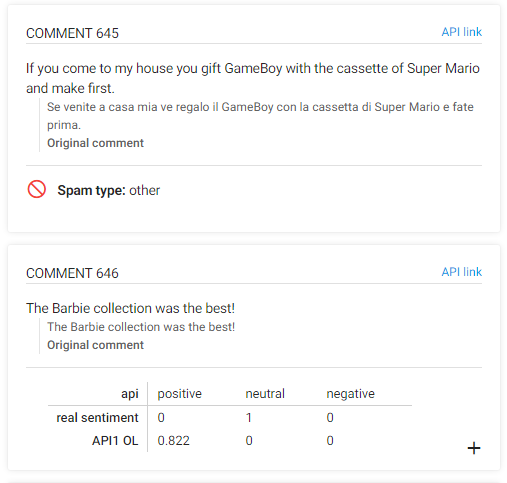
\includegraphics[width=1\textwidth]{04-framework/03-user-interface/images/comment_fragment.png}
	\caption[Comment Fragment]{Comment Fragment \label{fig:comment-fragment}}
\end{figure}

Keeping in mind that most preferred way of representing data is though visualization, we have decided to show sentiment scores though pie charts. Fragment that contains the chart is located on the right side of the web page. The chart fragment contains two pie charts, one representing statistics related to real sentiment score and second representing statistics related to sentiment score of chosen API as shown in the figure 4.5. User is able to choose between different API in order to visually compare them with real sentiment scores.

\newpage

\begin{figure}[ht]
	\centering	
	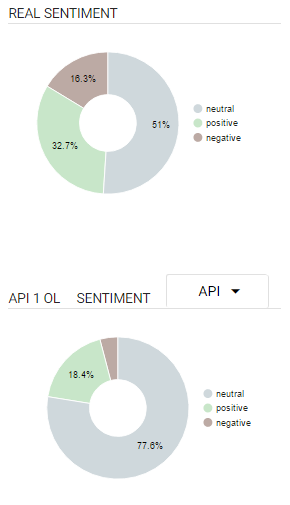
\includegraphics[width=0.5\textwidth]{04-framework/03-user-interface/images/pie_chart.png}
	\caption[Chart representation of sentiment score]{Chart representation of sentiment score \label{fig:pie-fragment}}
\end{figure}

Navigation to Stats tab, we are showing how we have calculated the accuracy of APIs, listed how many samples we have conducted the research on and listed percentage of negative, positive and neutral real sentiment comments. This webpage is giving opportunity to the user to see tabular representation of statistical results of each API with or without emojis, API with data translated in English and results taking into consideration the spam filters. Such tabular view has been enclosed below this paragraph. 

\begin{figure}[ht]
	\centering
	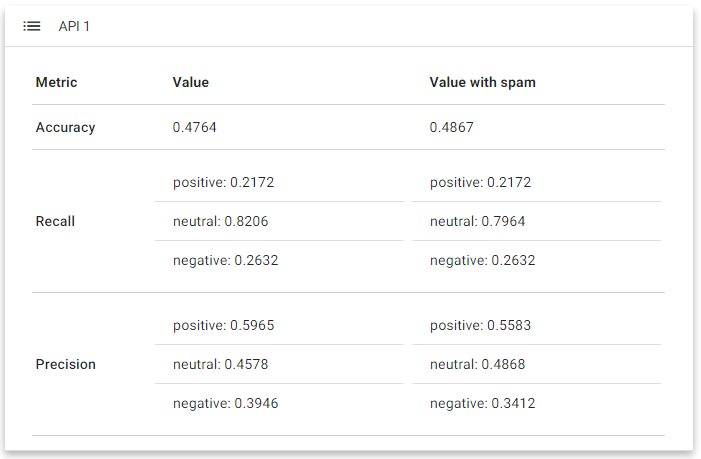
\includegraphics[width=0.8\textwidth]{04-framework/03-user-interface/images/stats.png}
	\caption[Tabular representation of statistical results for an API]{Tabular representation of statistical results for an API \label{fig:stats}}
\end{figure}

\newpage

\subsection{JSON REST API UI}

This section represents the data in JSON form using Django REST Framework. The used framework has brought us to having a browsable Web API in few steps. Following official documentation we were able to define all the relations between our entities and easily retrieve needed data. One of few views we are able to reach is shown on the figure below.

\begin{figure}[ht]
	\centering
	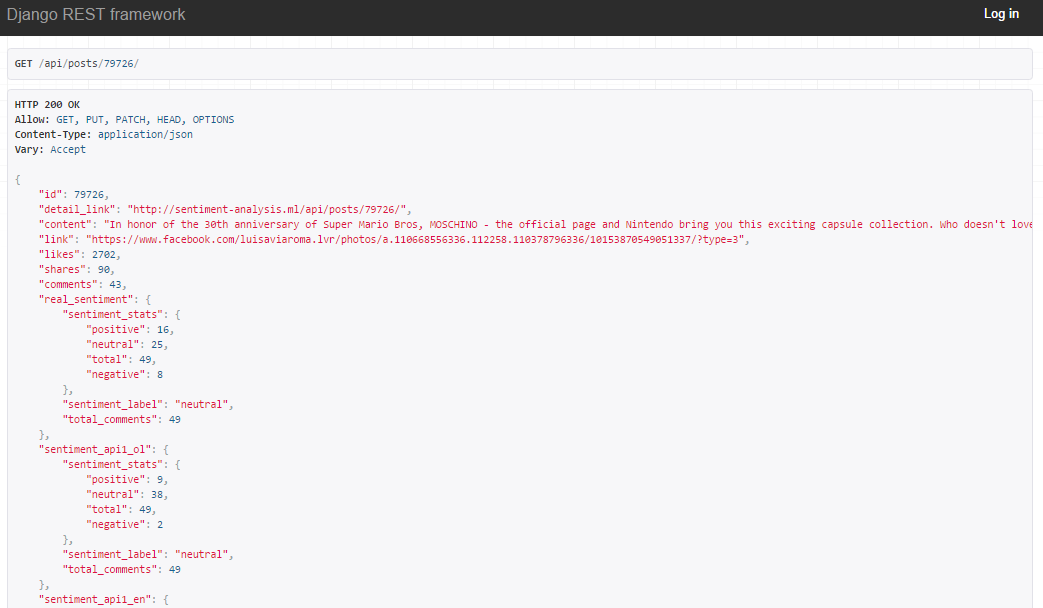
\includegraphics[width=0.8\textwidth]{04-framework/03-user-interface/images/django_api.png}
	\caption[JSON representation]{JSON representation \label{fig:django-api}}
\end{figure}

% --- CHAPTER RESULTS ---
\chapter{Results\label{ch:results}}
-- accuracy only of comments containing emojis vs only of the ones in plain text
-- accuracy only of comments originally in englich vs only of the ones translated

For the sake of completeness, below are the definitions used to calculate those 3 metrics.
Accuracy is the simplest of all metrics as it is just the fraction of correctly classified comment sentiments.
\[Accuracy = \frac{number\ of\ correct\ prediction}{total\ number \ of\ comments}\]

Precision and recall, on the other hand, are a bit more complex to understand and are calculated separately for each sentiment label $ \in \{ positive, negative, neutral \}$. 
They use concepts such as $True\ Positive$, $False\ Positive$  and $False\ Negative$.
In the context of out framework, these concepts are calculated as:
\begin{description}
 \item[True Positive] 
 correctly predicted labels
correctly identified like pairs {real sentiment, predicted sentiment} 
 {positive,positive}, {negative negative}
 \begin{description}
 \item[One] first item
 \item[Two] second item
 \item[Three] third item
\end{description}

 \item[False Positive]  
 number of times it didn't predict the label when it should have
 incorrectly identified {negative, neutral}
 \item[False negative] 
 umber of times it predicted the label when it shouldn't have 
\end{description}

Recall is the proportion of {positive, negative, neutral} comments were actually predicted as {positive, negative, neutral}. In other words, out of all the {positive, negative, neutral} examples, what fraction did the classifier pick up?
\[Recall = \frac{TP}{TP + FN }\]


Precision is the proportion of labels that were predicted as {positive,negative, neutral} actually are {positive,negative, neutral}. In other words, out of all the examples the classifier labeled as {positive,negative, neutral}, what fraction were correct?
\[Precision = \frac{TP}{TP + FP }\]

% --- CHAPTER CONCUSION ---
\chapter{Conclusion\label{ch:conclusion}}
In this final chapter we will summarize all the reasons for involving in such project, as well as the main contributions of the same. After listing the results we will address possible future improvements.

Nowadays with emerging markets and information flow it has become a necessity to try to predict future trends. Thus, companies are processing information luring through Internet with hope they will make a right choice. Big role in company's marketing strategy are social media channels, such as Facebook, Twitter or Instagram. Recognizing the potential use of customers input on the Web, companies have started gathering data related to their online advertisements. Logically, next step was to find a proper way of processing the data in order to discover certain correlations that could guide their production planning. One of recent methods for doing so is called sentiment analysis.

Our report consists of describing current trends in the field of sentiment analysis and how it is applied in business. Showing the reasons for using such method has brought us to idea of investigating about available open source solutions. We have tried to make a comparison with some of the most known sentiment analysis APIs on a given dataset which consists of Facebook comments related to a certain post about fashion industry products. 


% --- CHAPTER FUTURE WORK ---
\chapter{Future work\label{ch:future-work}}
\section{Connecting two mining approaches – Applying clustering in sentiment analysis}

One of newer ideas in area of sentiment analysis is using clustering algorithms in order to obtain better sentiment analysis results. Let's start with explaining what is clustering. Clustering is a method of splitting datasets into subsets of similar items based on the content of the items. In our case this would be splitting different post sentences in the same "basket" depending on the content, which would result in groups of sentences talking about a similar product feature (product aspect). 
Clustering is an unsupervised learning method, which means that items are split in separate groups only based on similarity value calculated by its features (in this case the content of the posts). Difference from classification method, where a model will be trained based on "past data", clustering method is based mostly on choosing an appropriate similarity measure. Other difference is that as output of classification your dataset is labeled with a class attribute, and in case of clustering, output is subsets of items. 

Applying clustering based sentiment analysis, we might obtain high accuracy results. The process contains few steps: 
\begin{enumerate}
	\item Data gathering
	\item Data cleaning
	\item Computing the Term Frequency and Inverse Document Frequency
	\item Applying K-means clustering algorithm
	\item Sentiment Analysis Engine
\end{enumerate}

After the data is gathered, it would be ideally to find an automatic data cleaning method that will remove all the outliers from the dataset. When obtaining relatively noisy free data we should perform TF-IDF in order to determine "keywords" in the content that could possibly represent a feature of an analyzed product. TF stands for Term Frequency, represents how many times a term occurs in a document. IDF stands for Inverse Document Frequency, and represents how common is a term in all documents. 
After determining the "keywords", we can have an idea of how many clusters we should expect in our dataset. This could be an input to the K-means algorithm, thus K-means chooses k random points as initial centroids and assigns all other points to the nearest centroid. Next step of the algorithm is re-centering the current centering. The process repeats until the next iteration produces same result as the previous iteration. Output of clustering method is set of clusters, where each cluster contains similar sentences. 

Output of the clustering step represents an input to the sentiment analysis engine. Each cluster is inserted in the engine to determine sentiment of people on a particular feature of the product.
Applied to our problem domain, the steps would go like so:
On each comment related to post, we would do data preprocessing, removing noisy data from the comment. Afterwards determining keywords in the comment related to the post. For example comment describing customers experience after using the product, such as a customer commenting on the fabric, quality, and color of the blouse. As input in K-mean we would have three aspects of product, in our case k would be 3. K-means would group all comment sentences related to each of the product features (quality, fabric and color). Afterwards, we apply the sentiment analysis on each cluster and obtain a sentiment value. This way we could calculate the overall sentiment value joining the cluster sentiment values, thus obtaining higher accuracy results.

Downsides of this approach:
\begin{enumerate}
	\item Applying method on large scale data
	\item Eliminating noisy data from social media content should usually involve human interaction
	\item Weaknesses of K-means method
\end{enumerate}

\section{Spam detection}

As one of the future improvements could be finding a better method for spam detection in order to filter out noisy comments that could give us less accurate sentiment estimation.  How could we differ spam from comments that are related to a post? Spam is an unwanted content appearing in the stream of comments. By unwanted content we assume content not related to the post or any other comments of the post. For example, URLs leading to third party web pages used as advertisements or a person that is tagged without any other information about the post. It is in our favor to try to remove such content from the analysis set which could lead to better sentiment estimation. 

We can look at spam detection as one of data preprocessing techniques. Currently we have used Akismet for spam detection; it is a web service for recognizing spam comments. To be able to estimate effectiveness of Akismet service, we have determined manually if a comment is a spam or not. Having a small comment dataset it was not time consuming to manually analyze the comments. After the analysis we have calculated the accuracy of chosen spam detection method. Unfortunately, the results have shown that on our dataset Akismet was not so effective.

\section{Out of the black box – Training a model}

Our project has been based on testing different APIs for sentiment analysis and determining which of the used APIs has given the best results. Using APIs as they are could be imagined as using a tool without knowing what is actually going on inside it. This way we could not tune the algorithm to suit our problem domain. By going out of the box, we could build a model that would provide us with better sentiment analysis results. 

Training a model can be seen as producing a function that applied on future data could give sentiment “class label”, in our case positive, negative or neutral value, with higher accuracy then the used APIs. The process of building a model consists of training a model on training set, validating the model and afterwards testing in on the test set. 



% --- CHAPTER BIBLIOGRAPHY ---
\bibliographystyle{ieeetr}
\bibliography{bibliography}
\addcontentsline{toc}{chapter}{Bibliography}


\end{document}
